\documentclass[aspectratio=169,11pt]{beamer}
\usetheme{default}
\setbeamertemplate{navigation symbols}{}
\setbeamertemplate{footline}{%
  \hfill\insertframenumber/\inserttotalframenumber\hspace*{4pt}\vspace{2pt}%
}
\usepackage{lmodern}
\usepackage[most]{tcolorbox}
\usepackage{listings}
\usepackage{tikz}
\usetikzlibrary{arrows.meta,positioning,shapes.geometric,fit,backgrounds}
\usepackage{booktabs}
\usepackage{hyperref}

\definecolor{lcgreen}{HTML}{2E7D32}
\definecolor{lcblue}{HTML}{1565C0}
\definecolor{lcorange}{HTML}{EF6C00}
\definecolor{lcred}{HTML}{C62828}
\definecolor{codebg}{HTML}{F5F5F5}
\definecolor{docgray}{gray}{0.55}

\newtcolorbox{conceptbox}[1][]{colback=yellow!20,colframe=yellow!60!black,title=#1,fonttitle=\bfseries,top=1pt,bottom=1pt,left=3pt,right=3pt}
\newtcolorbox{warningbox}[1][]{colback=red!15,colframe=red!60!black,title=#1,fonttitle=\bfseries,top=1pt,bottom=1pt,left=3pt,right=3pt}
\newtcolorbox{tipbox}[1][]{colback=green!10,colframe=green!50!black,title=#1,fonttitle=\bfseries,top=1pt,bottom=1pt,left=3pt,right=3pt}
\newtcolorbox{codebox}[1][]{colback=blue!10,colframe=blue!40!black,title=#1,fonttitle=\bfseries,top=1pt,bottom=1pt,left=3pt,right=3pt}

\lstset{
  basicstyle=\ttfamily\tiny,
  backgroundcolor=\color{codebg},
  breaklines=true,
  frame=single,
  rulecolor=\color{blue!40!black},
  keywordstyle=\color{lcblue}\bfseries,
  stringstyle=\color{lcgreen},
  commentstyle=\color{docgray}\itshape,
  language=Python,
  showstringspaces=false,
  tabsize=2,
  xleftmargin=1pt,
  xrightmargin=1pt,
  aboveskip=1pt,
  belowskip=1pt,
}

\newcommand{\docref}[1]{{\scriptsize\color{docgray}[Docs: #1]}}

\title{Section 08: Embeddings, Vector Stores \& Retrievers}
\subtitle{LangChain v1.2.x (March 2026)}
\author{LangChain Documentation}
\date{}

\begin{document}

\begin{frame}
  \titlepage
\end{frame}

% Frame 2: Table of Contents
\begin{frame}{Roadmap: Embeddings, Vector Stores \& Retrievers}
  \begin{itemize}
    \setlength{\itemsep}{1pt}
    \item \textbf{Mental Model:} The semantic search pipeline
    \item \textbf{Embeddings:} Converting text to vectors, similarity
    \item \textbf{The Embeddings Interface:} Core methods and providers
    \item \textbf{Vector Stores:} Purpose, implementations, operations
    \item \textbf{Retrievers:} Fetching relevant documents
    \item \textbf{Advanced Patterns:} Multi-query, compression, ensemble
    \item \textbf{Performance \& Pitfalls:} Real-world considerations
  \end{itemize}
  \vspace{0.05cm}
  \textcolor{lcblue}{\textbf{Goal:}} Build production-ready retrieval pipelines
\end{frame}

% Frame 3: Mental Model - Semantic Search Pipeline
\begin{frame}{Mental Model: The Semantic Search Pipeline}
  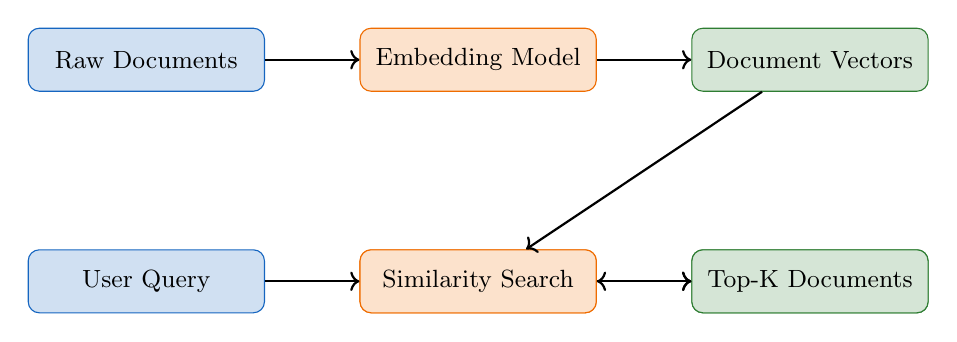
\begin{tikzpicture}[
    node distance=1.2cm,
    every node/.style={draw, rounded corners, minimum width=3cm, minimum height=0.8cm, text centered, font=\small},
    box/.style={fill=lcblue!20, draw=lcblue},
    process/.style={fill=lcorange!20, draw=lcorange},
    output/.style={fill=lcgreen!20, draw=lcgreen}
  ]
    % Documents phase
    \node[box] (docs) {Raw Documents};
    \node[process, right=of docs] (embed) {Embedding Model};
    \node[output, right=of embed] (vectors) {Document Vectors};

    % Query phase
    \node[box, below=2cm of docs] (query) {User Query};
    \node[process, right=of query] (qembed) {Embedding Model};
    \node[output, right=of qembed] (qvector) {Query Vector};

    % Retrieval phase
    \node[process, below=2cm of embed] (search) {Similarity Search};
    \node[output, right=of search] (results) {Top-K Documents};

    % Edges
    \draw[->, thick] (docs) -- (embed);
    \draw[->, thick] (embed) -- (vectors);
    \draw[->, thick] (query) -- (qembed);
    \draw[->, thick] (qembed) -- (qvector);
    \draw[->, thick] (vectors) -- (search);
    \draw[->, thick] (qvector) -- (search);
    \draw[->, thick] (search) -- (results);
  \end{tikzpicture}
  \vspace{0.05cm}
  \begin{conceptbox}[Key Insight]
    Documents and queries are converted to vectors in the \emph{same} embedding space.\\
    Similarity = semantic relatedness in vector space.
  \end{conceptbox}
\end{frame}

% Frame 4: What Are Embeddings?
\begin{frame}{What Are Embeddings? Text \textrightarrow\ Vectors}
  \begin{itemize}
    \setlength{\itemsep}{1pt}
    \item \textbf{Embedding:} A dense vector representation of text
    \item Captures \emph{semantic meaning}, not just bag-of-words
    \item Example dimensions: 384 (small), 1536 (OpenAI text-embedding-3-small), 3072 (text-embedding-3-large)
  \end{itemize}

  \vspace{0.05cm}
  \begin{center}
    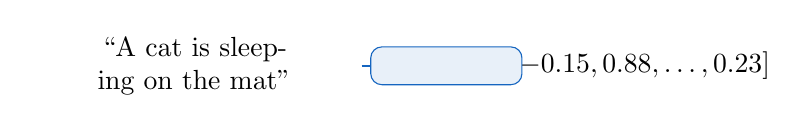
\begin{tikzpicture}[scale=0.8]
      \node[text width=4cm, align=center] (text) {``A cat is sleeping on the mat''};
      \draw[->, thick, lcblue] (text) -- (3, 0);
      \node[right=of text] (vec) {$[0.42, -0.15, 0.88, \ldots, 0.23]$};
      \draw[rounded corners, fill=lcblue!10, draw=lcblue] (2.8, -0.3) rectangle (5.2, 0.3);
    \end{tikzpicture}
  \end{center}

  \vspace{0.05cm}
  \begin{tipbox}[Semantic Similarity]
    \textbf{``A cat rests on the floor''} produces a \emph{nearby} vector $\rightarrow$ high cosine similarity.\\
    \textbf{``The weather is sunny today''} produces a \emph{distant} vector $\rightarrow$ low cosine similarity.
  \end{tipbox}
\end{frame}

% Frame 5: The Embeddings Interface
\begin{frame}[fragile,shrink=15]{The Embeddings Interface: Core Methods}
  \begin{conceptbox}[API Contract]
    All embedding providers implement the same interface:
  \end{conceptbox}

  \begin{lstlisting}
from langchain_core.embeddings import Embeddings

class Embeddings(ABC):
    """Abstract base for embedding models."""

    @abstractmethod
    def embed_documents(
        self, texts: List[str]
    ) -> List[List[float]]:
        """Embed a list of documents."""
        pass

    @abstractmethod
    def embed_query(self, text: str) -> List[float]:
        """Embed a single query string."""
        pass
  \end{lstlisting}

  \vspace{0.07cm}
  \docref{langchain-core.embeddings}
\end{frame}

% Frame 6: OpenAI Embeddings Setup
\begin{frame}[fragile]{OpenAIEmbeddings Setup and Usage}
  \begin{lstlisting}
import os
from langchain_openai import OpenAIEmbeddings

# Initialize with OPENAI_API_KEY environment variable
embeddings = OpenAIEmbeddings(
    model="text-embedding-3-small"
)

# Embed documents (batch)
docs = [
    "LangChain simplifies LLM application development",
    "Embeddings map text to vectors"
]
doc_vectors = embeddings.embed_documents(docs)
print(f"Doc vectors: {len(doc_vectors)} x {len(doc_vectors[0])}")

# Embed a single query
query = "What is semantic search?"
query_vector = embeddings.embed_query(query)
print(f"Query vector dimension: {len(query_vector)}")
  \end{lstlisting}

  \vspace{0.07cm}
  \docref{langchain-openai.embeddings}
\end{frame}

% Frame 7: Other Embedding Providers
\begin{frame}[fragile]{Other Embedding Providers}
  \begin{columns}
    \column{0.48\textwidth}
    \textbf{Anthropic Embeddings:}
    \begin{lstlisting}[basicstyle=\ttfamily\tiny]
from langchain_anthropic import \
  AnthropicEmbeddings
emb = AnthropicEmbeddings(
  model="claude-3-5-sonnet-20241022"
)
    \end{lstlisting}

    \vspace{0.07cm}
    \textbf{HuggingFace (remote):}
    \begin{lstlisting}[basicstyle=\ttfamily\tiny]
from langchain_huggingface import \
  HuggingFaceEmbeddings
emb = HuggingFaceEmbeddings(
  model_name="all-MiniLM-L6-v2"
)
    \end{lstlisting}

    \column{0.48\textwidth}
    \textbf{Ollama (local):}
    \begin{lstlisting}[basicstyle=\ttfamily\tiny]
from langchain_ollama import OllamaEmbeddings
emb = OllamaEmbeddings(
  model="nomic-embed-text"
)
    \end{lstlisting}

    \vspace{0.07cm}
    \textbf{Cohere:}
    \begin{lstlisting}[basicstyle=\ttfamily\tiny]
from langchain_cohere import CohereEmbeddings
emb = CohereEmbeddings(
  model="embed-english-v3.0"
)
    \end{lstlisting}
  \end{columns}

  \vspace{0.05cm}
  \begin{warningbox}[Note]
    Local embeddings (HuggingFace, Ollama) = free but slower. Cloud = faster but costs per API call.
  \end{warningbox}
\end{frame}

% Frame 8: Embedding Models Comparison
\begin{frame}{Comparison: Embedding Models (March 2026)}
  \small
  \begin{tabular}{llccc}
    \toprule
    \textbf{Model} & \textbf{Provider} & \textbf{Dim} & \textbf{Cost} & \textbf{Quality} \\
    \midrule
    text-embedding-3-small & OpenAI & 1536 & \$0.02/1M & High \\
    text-embedding-3-large & OpenAI & 3072 & \$0.13/1M & Very High \\
    all-MiniLM-L6-v2 & HF (local) & 384 & Free & Medium \\
    all-mpnet-base-v2 & HF (local) & 768 & Free & High \\
    nomic-embed-text-1.5 & Ollama & 768 & Free & High \\
    embed-english-v3.0 & Cohere & 1024 & \$0.10/1M & Very High \\
    Claude-3.5-Sonnet & Anthropic & 1024 & \$3/1M tokens & Very High \\
    \bottomrule
  \end{tabular}

  \vspace{0.05cm}
  \begin{tipbox}[Selection Guide]
    \textbf{Prototyping:} all-MiniLM-L6-v2 (fast, free)\\
    \textbf{Production:} text-embedding-3-small (quality/cost)\\
    \textbf{Privacy:} Ollama local embeddings
  \end{tipbox}
\end{frame}

% Frame 9: What Are Vector Stores?
\begin{frame}{What Are Vector Stores? Purpose \& Design}
  \begin{conceptbox}[Definition]
    A \textbf{vector store} is a database optimized for:
    \begin{itemize}
    \setlength{\itemsep}{1pt}
      \item Storing high-dimensional dense vectors
      \item Fast \emph{approximate} nearest-neighbor (ANN) search
      \item Associating vectors with metadata (source, page, etc.)
    \end{itemize}
  \end{conceptbox}

  \vspace{0.05cm}
  \textbf{How it works:}
  \begin{enumerate}
    \setlength{\itemsep}{0pt}
    \item Index documents: convert texts to vectors, build search structure
    \item Query: embed user query, find nearest vectors
    \item Return: top-K matching documents with metadata
  \end{enumerate}

  \vspace{0.05cm}
  \begin{warningbox}[ANN vs Exact Search]
    Vector stores use \emph{approximate} search (faster, slightly less accurate) not exhaustive search.
  \end{warningbox}
\end{frame}

% Frame 10: FAISS - In-Memory Vector Store
\begin{frame}[fragile]{FAISS: In-Memory Vector Store}
  \begin{lstlisting}[basicstyle=\ttfamily\tiny]
from langchain_community.vectorstores \
  import FAISS
embeddings = OpenAIEmbeddings()
documents = ["RAG applications", "semantic search",
  "index documents efficiently"]
vector_store = FAISS.from_texts(
  documents, embeddings)
results = vector_store.similarity_search(
  "semantic search", k=2)
  \end{lstlisting}

  \textbf{Pros:} Fast, in-memory. \textbf{Cons:} Not persistent.
\end{frame}

% Frame 11: Chroma - Persistent Local Vector Store
\begin{frame}[fragile]{Chroma: Persistent Local Vector Store}
  \begin{lstlisting}[basicstyle=\ttfamily\tiny]
from langchain_chroma import Chroma
embeddings = OpenAIEmbeddings()
vector_store = Chroma(
  collection_name="my_docs",
  embedding_function=embeddings,
  persist_directory="./chroma_db"
)
vector_store.add_documents([
  Document(page_content="...",
    metadata={"source": "doc1.pdf"})
])
results = vector_store.similarity_search("query")
  \end{lstlisting}

  \textbf{Pros:} Persistent, local. \textbf{Cons:} Limited scale.
\end{frame}

% Frame 12: Pinecone - Managed Cloud Vector Store
\begin{frame}[fragile]{Pinecone: Managed Cloud Vector Store}
  \begin{lstlisting}[basicstyle=\ttfamily\tiny]
from langchain_pinecone import PineconeVectorStore
embeddings = OpenAIEmbeddings()
vector_store = PineconeVectorStore(
  index_name="my-index",
  embedding=embeddings,
  namespace="production"
)
vector_store.add_documents(documents)
results = vector_store.similarity_search(
  "machine learning", k=5
)
  \end{lstlisting}

  \textbf{Pros:} Managed, scales. \textbf{Cons:} Cost.
\end{frame}

% Frame 13: Vector Store Operations
\begin{frame}[fragile]{Common Vector Store Operations}
  \begin{lstlisting}
from langchain_chroma import Chroma

vector_store = Chroma(...)

# 1. Add documents
vector_store.add_documents(docs)

# 2. Add texts with explicit IDs
ids = vector_store.add_texts(
    ["text1", "text2"],
    ids=["id1", "id2"]
)

# 3. Similarity search (top-k)
results = vector_store.similarity_search(
    "query", k=3
)

# 4. Similarity search with scores
results_with_scores = \
  vector_store.similarity_search_with_score(
    "query", k=3
)
for doc, score in results_with_scores:
    print(f"Score: {score:.3f}, Content: {doc.page_content}")
  \end{lstlisting}

  \vspace{0.07cm}
  \docref{vector-stores}
\end{frame}

% Frame 14: Vector Store as Retriever
\begin{frame}[fragile]{Vector Store as Retriever: as\_retriever()}
  \begin{lstlisting}
from langchain_chroma import Chroma
from langchain_openai import OpenAIEmbeddings

embeddings = OpenAIEmbeddings()
vector_store = Chroma(embedding_function=embeddings)
vector_store.add_documents(documents)

# Convert to retriever interface
retriever = vector_store.as_retriever(
    search_type="similarity",
    search_kwargs={"k": 3}
)

# Use in chains
from langchain.chains import create_retrieval_chain
from langchain_openai import ChatOpenAI

llm = ChatOpenAI()
chain = create_retrieval_chain(retriever, llm)

result = chain.invoke({"input": "What is RAG?"})
print(result["answer"])
  \end{lstlisting}

  \docref{retrievers}
\end{frame}

% Frame 15: The Retriever Interface
\begin{frame}[shrink=8]{The Retriever Interface and How It Works}
  \begin{conceptbox}[Retriever API]
    All retrievers implement one core method:
    \begin{center}
      \texttt{get\_relevant\_documents(query: str) -> List[Document]}
    \end{center}
    Returns a list of documents ranked by relevance.
  \end{conceptbox}

  \vspace{0.05cm}
  \textbf{Key points:}
  \begin{enumerate}
    \setlength{\itemsep}{0pt}
    \item Retrievers are \emph{pluggable} — swap implementations without changing downstream code
    \item Input: a string query
    \item Output: ordered list of relevant \texttt{Document} objects
    \item Used by chains, agents, and RAG systems to fetch context
  \end{enumerate}

  \vspace{0.05cm}
  \begin{tipbox}[Design Benefit]
    Same interface works for vector stores, BM25, web search, databases, etc.\\
    Encourages composable, testable retrieval systems.
  \end{tipbox}
\end{frame}

% Frame 16: Similarity Search vs MMR
\begin{frame}[fragile]{Similarity Search vs MMR (Maximal Marginal Relevance)}
  \textbf{Similarity Search:} Returns documents most similar to query.
  \begin{lstlisting}[basicstyle=\ttfamily\tiny]
results = vector_store.similarity_search("topic", k=3)
# Returns: [doc_most_relevant, doc_2nd_relevant, doc_3rd_relevant]
  \end{lstlisting}

  \textbf{Problem:} Top results may be redundant (say the same thing).

  \vspace{0.07cm}
  \textbf{MMR:} Maximizes relevance \emph{and} diversity.
  \begin{lstlisting}[basicstyle=\ttfamily\tiny]
retriever = vector_store.as_retriever(
    search_type="mmr",
    search_kwargs={"k": 3, "fetch_k": 10}
)
results = retriever.get_relevant_documents("topic")
# fetch_k=10 candidates, return k=3 most diverse
  \end{lstlisting}

  \vspace{0.07cm}
  \begin{tipbox}[When to Use MMR]
    Use MMR for synthesis tasks (survey, comparison) where diversity matters.\\
    Use similarity search for direct QA where relevance is paramount.
  \end{tipbox}
\end{frame}

% Frame 17: Metadata Filtering in Retrievers
\begin{frame}[fragile]{Metadata Filtering in Retrievers}
  \begin{lstlisting}
from langchain_chroma import Chroma

vector_store = Chroma(...)

# Add documents with metadata
vector_store.add_documents([
    Document(
        page_content="...",
        metadata={"source": "arxiv.pdf", "year": 2024}
    ),
    Document(
        page_content="...",
        metadata={"source": "blog.md", "year": 2025}
    )
])

# Create retriever with metadata filter
retriever = vector_store.as_retriever(
    search_kwargs={
        "k": 3,
        "filter": {"year": 2025}  # Only 2025 docs
    }
)

results = retriever.get_relevant_documents("query")
  \end{lstlisting}

  \vspace{0.07cm}
  \textbf{Note:} Filter syntax varies by vector store (Chroma, Pinecone, etc.).
\end{frame}

% Frame 18: Multi-Query Retriever
\begin{frame}[fragile]{Multi-Query Retriever: Generating Multiple Search Queries}
  \begin{lstlisting}
from langchain.retrievers.multi_query import \
  MultiQueryRetriever
from langchain_chroma import Chroma
from langchain_openai import ChatOpenAI

vector_store = Chroma(...)
llm = ChatOpenAI()

# Wraps a base retriever
multi_query_retriever = MultiQueryRetriever.from_llm(
    retriever=vector_store.as_retriever(
      search_kwargs={"k": 2}
    ),
    llm=llm
)

# Generates 3 variants of the query
results = multi_query_retriever.get_relevant_documents(
    "What is embeddings?"
)
# Queries: "What is embeddings?", "How do embeddings work?", ...
  \end{lstlisting}

  \vspace{0.07cm}
  \begin{conceptbox}[Why Multi-Query?]
    Different phrasings of the same question retrieve different documents.\\
    More robust, fewer missed results.
  \end{conceptbox}
\end{frame}

% Frame 19: Contextual Compression Retriever
\begin{frame}[fragile]{Contextual Compression Retriever}
  \begin{lstlisting}
from langchain.retrievers import \
  ContextualCompressionRetriever
from langchain.retrievers.document_compressors \
  import LLMCompressor
from langchain_openai import ChatOpenAI
from langchain_chroma import Chroma

vector_store = Chroma(...)
llm = ChatOpenAI()

# Wraps base retriever with compression
compressor = LLMCompressor.from_llm(llm)
compression_retriever = \
  ContextualCompressionRetriever(
    base_compressor=compressor,
    base_retriever=vector_store.as_retriever(k=10)
  )

# Returns only relevant passages (not full docs)
results = compression_retriever.get_relevant_documents(
    "specific detail"
)
  \end{lstlisting}

  \vspace{0.07cm}
  \textbf{Benefit:} Reduces token usage by extracting only relevant passages.
\end{frame}

% Frame 20: Ensemble Retriever
\begin{frame}[fragile]{Ensemble Retriever: Combining Multiple Retrievers}
  \begin{lstlisting}
from langchain.retrievers import EnsembleRetriever
from langchain_chroma import Chroma
from langchain_community.retrievers import BM25Retriever

documents = [...]

# Retriever 1: Vector store (semantic)
chroma = Chroma.from_documents(documents, embeddings)
vector_retriever = chroma.as_retriever(k=2)

# Retriever 2: BM25 (keyword-based)
bm25_retriever = BM25Retriever.from_documents(documents)
bm25_retriever.k = 2

# Ensemble: Reciprocal Rank Fusion
ensemble = EnsembleRetriever(
    retrievers=[vector_retriever, bm25_retriever],
    weights=[0.5, 0.5]  # Equal importance
)

results = ensemble.get_relevant_documents("query")
  \end{lstlisting}

  \vspace{0.07cm}
  \textbf{Why:} Combines semantic + keyword strengths. More robust results.
\end{frame}

% Frame 21: TikZ Diagram - Indexing Pipeline
\begin{frame}{Indexing Pipeline Visualization}
  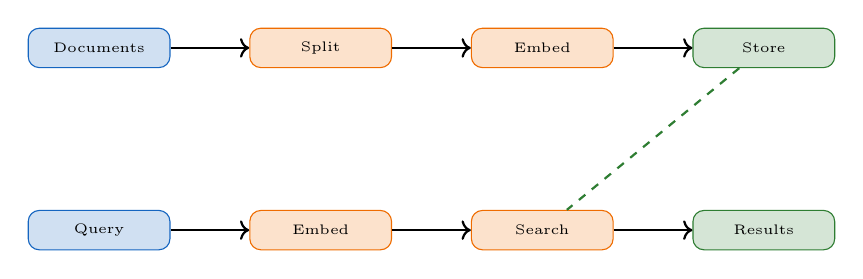
\begin{tikzpicture}[
    node distance=1.0cm,
    every node/.style={draw, rounded corners, minimum width=1.8cm, minimum height=0.5cm, text centered, font=\tiny},
    input/.style={fill=lcblue!20, draw=lcblue},
    process/.style={fill=lcorange!20, draw=lcorange},
    storage/.style={fill=lcgreen!20, draw=lcgreen}
  ]
    \node[input] (raw) {Documents};
    \node[process, right=of raw] (split) {Split};
    \node[process, right=of split] (emb) {Embed};
    \node[storage, right=of emb] (store) {Store};

    \draw[->, thick] (raw) -- (split);
    \draw[->, thick] (split) -- (emb);
    \draw[->, thick] (emb) -- (store);

    \node[input, below=1.8cm of raw] (query) {Query};
    \node[process, right=of query] (qemb) {Embed};
    \node[process, right=of qemb] (search) {Search};
    \node[storage, right=of search] (results) {Results};

    \draw[->, thick] (query) -- (qemb);
    \draw[->, thick] (qemb) -- (search);
    \draw[dashed, thick, lcgreen] (store) -- (search);
    \draw[->, thick] (search) -- (results);
  \end{tikzpicture}

  \textbf{Key:} Same embedding for docs and queries.
\end{frame}

% Frame 22: Retrieval Pipeline in Detail
\begin{frame}{Retrieval Pipeline}
  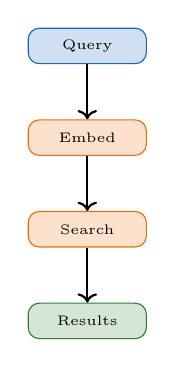
\begin{tikzpicture}[scale=0.85,
    node distance=0.7cm,
    every node/.style={draw, rounded corners, minimum width=1.5cm, minimum height=0.45cm, text centered, font=\tiny},
    input/.style={fill=lcblue!20, draw=lcblue},
    process/.style={fill=lcorange!20, draw=lcorange},
    output/.style={fill=lcgreen!20, draw=lcgreen}
  ]
    \node[input] (query) {Query};
    \node[process, below=of query] (embed) {Embed};
    \node[process, below=of embed] (search) {Search};
    \node[output, below=of search] (final) {Results};

    \draw[->, thick] (query) -- (embed);
    \draw[->, thick] (embed) -- (search);
    \draw[->, thick] (search) -- (final);
  \end{tikzpicture}

  \textbf{Steps:} Embed query $\to$ Find neighbors $\to$ Return results
\end{frame}

% Frame 23: Performance Considerations - Index Size
\begin{frame}{Performance Considerations: Index Size}
  \begin{itemize}
    \setlength{\itemsep}{1pt}
    \item \textbf{Number of documents:} 1K (FAISS OK), 1M+ (Pinecone needed)
    \item \textbf{Vector dimensions:} Higher = more expressive but slower (1536 is practical maximum)
    \item \textbf{Search latency:} Trade-off between accuracy and speed
      \begin{itemize}
    \setlength{\itemsep}{1pt}
        \item Exact search: O(n) — accurate but slow
        \item HNSW/IVF (approximate): O(log n) — fast but lossy
      \end{itemize}
  \end{itemize}

  \vspace{0.05cm}
  \begin{conceptbox}[Memory Cost]
    Storage = (num\_docs × dimensions × 4 bytes) + metadata\\
    Example: 1M docs × 1536 dims × 4 bytes = \textbf{6 GB}
  \end{conceptbox}

  \vspace{0.07cm}
  \begin{tipbox}[Optimization Tips]
    Chunk documents (e.g., 300-token chunks) to balance coverage and retrieval precision.\\
    Use quantization (8-bit) to reduce memory 4x at slight accuracy cost.
  \end{tipbox}
\end{frame}

% Frame 24: Performance - Embedding Cost
\begin{frame}{Performance Considerations: Embedding Cost}
  \textbf{Pricing breakdown (OpenAI text-embedding-3-small):}
  \begin{itemize}
    \setlength{\itemsep}{1pt}
    \item \$0.02 per 1 million tokens
    \item Indexing: ~4000 words = 5000 tokens = \$0.0001
    \item For 100K documents: \textbf{\$10 one-time cost}
  \end{itemize}

  \vspace{0.05cm}
  \textbf{Query embedding cost:}
  \begin{itemize}
    \setlength{\itemsep}{1pt}
    \item Each query = ~100 tokens = \$0.000002
    \item Negligible at scale
  \end{itemize}

  \vspace{0.05cm}
  \begin{warningbox}[Cost Optimization]
    Cache embeddings (don't re-embed the same documents).\\
    Use free local embeddings (HuggingFace) if cost is critical.\\
    Batch embedding calls for efficiency.
  \end{warningbox}
\end{frame}

% Frame 25: Performance - Search Latency
\begin{frame}{Performance Considerations: Search Latency}
  \textbf{Typical latencies:}
  \begin{itemize}
    \setlength{\itemsep}{1pt}
    \item \textbf{FAISS (in-memory):} 1--10 ms for 100K docs
    \item \textbf{Chroma (disk-backed):} 10--100 ms
    \item \textbf{Pinecone (cloud):} 100--500 ms (including network)
  \end{itemize}

  \vspace{0.05cm}
  \textbf{Optimization levers:}
  \begin{enumerate}
    \setlength{\itemsep}{0pt}
    \item Reduce \texttt{k} (fetch fewer results)
    \item Use quantization (trade accuracy for speed)
    \item Shard index across multiple machines
    \item Cache frequent queries
  \end{enumerate}

  \vspace{0.05cm}
  \begin{tipbox}[Production SLA]
    Target < 200 ms end-to-end (embedding + search + LLM call).\\
    Use ensemble of retrievers + background indexing for <100 ms.
  \end{tipbox}
\end{frame}

% Frame 26: Common Pitfall 1 - Dimension Mismatch
\begin{frame}[fragile]{Common Pitfall 1: Dimension Mismatch}
  \begin{warningbox}[Error Scenario]
    You index documents with embedding model A (1536 dims) but query with model B (384 dims).
  \end{warningbox}

  \vspace{0.05cm}
  \textbf{Problem:} Similarity computation fails or returns meaningless results.

  \vspace{0.05cm}
  \textbf{Solution:}
  \begin{lstlisting}[basicstyle=\ttfamily\tiny]
# WRONG: Different models for indexing and querying
index_embeddings = OpenAIEmbeddings(model="text-embedding-3-small")  # 1536
query_embeddings = HuggingFaceEmbeddings(model="all-MiniLM-L6-v2")  # 384

# RIGHT: Use same model consistently
embeddings = OpenAIEmbeddings(model="text-embedding-3-small")
vector_store = Chroma(embedding_function=embeddings)
retriever = vector_store.as_retriever()
  \end{lstlisting}

  \begin{tipbox}[Best Practice]
    Define embedding model once, pass it to all components.
  \end{tipbox}
\end{frame}

% Frame 27: Common Pitfall 2 - Missing Metadata
\begin{frame}[fragile,shrink=20]{Common Pitfall 2: Missing or Incomplete Metadata}
  \begin{warningbox}[Error Scenario]
    You index documents without storing source information. Later, results include relevance scores but you don't know where they came from.
  \end{warningbox}

  \vspace{0.05cm}
  \textbf{Solution:}
  \begin{lstlisting}[basicstyle=\ttfamily\tiny]
from langchain_core.documents import Document

# WRONG: No metadata
docs = [Document(page_content="...")]

# RIGHT: Include rich metadata
docs = [
    Document(
        page_content="...",
        metadata={
            "source": "arxiv:2310.04567",
            "page": 3,
            "date": "2023-10-01",
            "author": "Smith et al."
        }
    )
]
vector_store.add_documents(docs)
  \end{lstlisting}

  \begin{tipbox}[Metadata Strategy]
    Always include: source, page/section, date.\\
    Optional: author, category, tags for filtering.
  \end{tipbox}
\end{frame}

% Frame 28: Common Pitfall 3 - Wrong Similarity Metric
\begin{frame}[fragile]{Common Pitfall 3: Wrong Similarity Metric}
  \begin{itemize}
    \setlength{\itemsep}{1pt}
    \item \textbf{Cosine Similarity:} Standard (most vector stores), works for normalized embeddings
    \item \textbf{Euclidean Distance:} Less common, requires careful scaling
    \item \textbf{Dot Product:} Fast but requires pre-normalized vectors
  \end{itemize}

  \vspace{0.05cm}
  \begin{warningbox}[Issue]
    If embeddings are \texttt{float32} unnormalized, Euclidean distance inflates with dimension count.
  \end{warningbox}

  \vspace{0.05cm}
  \textbf{Best practice:} Stick with cosine similarity (default in most libraries).
  \begin{lstlisting}[basicstyle=\ttfamily\tiny]
# Most vector stores default to cosine
results = vector_store.similarity_search(query, k=3)
# Equivalent to: cos(query_vec, doc_vec)
  \end{lstlisting}

  \begin{tipbox}[Note]
    OpenAI embeddings are normalized; cosine similarity equals dot product.\\
    No need to manually normalize.
  \end{tipbox}
\end{frame}

% Frame 29: Common Pitfall 4 - Ignoring Chunking
\begin{frame}[fragile]{Common Pitfall 4: Ignoring Document Chunking}
  \begin{warningbox}[Problem]
    If you index entire PDFs (10K tokens each) without splitting, retrieval returns entire documents.\\
    Context may be too large for LLM, includes irrelevant sections.
  \end{warningbox}

  \vspace{0.05cm}
  \textbf{Solution: Chunk before indexing}
  \begin{lstlisting}[basicstyle=\ttfamily\tiny]
from langchain_text_splitters import RecursiveCharacterTextSplitter

splitter = RecursiveCharacterTextSplitter(
    chunk_size=512,
    chunk_overlap=50
)
chunks = splitter.split_documents(docs)
vector_store.add_documents(chunks)
  \end{lstlisting}

  \begin{tipbox}[Chunk Guidelines]
    Typical: 256--1024 tokens per chunk.\\
    Overlap: 50--100 tokens (preserves context at boundaries).\\
    Adjust based on domain (code needs longer chunks than prose).
  \end{tipbox}
\end{frame}

% Frame 30: Production Checklist
\begin{frame}{Production Readiness Checklist}
  \begin{enumerate}
    \setlength{\itemsep}{0pt}
    \item \textbf{Embedding Model:} Fixed and documented across all services
    \item \textbf{Vector Store Persistence:} Backups, version control for index
    \item \textbf{Metadata Completeness:} Every document has source, date, category
    \item \textbf{Chunk Size Tuning:} Tested on representative corpus
    \item \textbf{Search Quality:} Manual evaluation of top-K results
    \item \textbf{Latency Monitoring:} Track p50, p95, p99 search times
    \item \textbf{Cost Tracking:} Monitor embedding API calls and storage costs
    \item \textbf{Freshness Strategy:} Plan for incremental indexing, re-indexing frequency
    \item \textbf{Error Handling:} Graceful degradation if vector store is unavailable
    \item \textbf{Security:} Secure API keys, data encryption at rest and in transit
  \end{enumerate}

  \vspace{0.05cm}
  \docref{production-guide}
\end{frame}

% Frame 31: Real-World Example - RAG Chain
\begin{frame}[fragile]{Real-World Example: RAG Chain}
  \scriptsize
  \begin{lstlisting}[basicstyle=\ttfamily\tiny]
embeddings = OpenAIEmbeddings()
vector_store = Chroma(embedding_function=embeddings)
vector_store.add_documents(my_docs)
retriever = vector_store.as_retriever(k=3)
prompt = ChatPromptTemplate.from_messages([
  ("system","Use context: {context}"),
  ("user","{input}")
])
llm = ChatOpenAI()
chain = create_retrieval_chain(
  retriever, create_stuff_chain(llm,prompt))
result = chain.invoke({"input": "Q?"})
  \end{lstlisting}
\end{frame}

% Frame 32: Real-World Example - Hybrid Search
\begin{frame}[fragile]{Real-World Example: Hybrid Search}
  \begin{lstlisting}[basicstyle=\ttfamily\tiny]
embeddings = OpenAIEmbeddings()
vector = Chroma.from_documents(docs, embeddings)
bm25 = BM25Retriever.from_documents(docs)
ensemble = EnsembleRetriever(
  retrievers=[vector.as_retriever(k=3), bm25],
  weights=[0.5, 0.5])
results = ensemble.get_relevant_documents("query")
  \end{lstlisting}

  \textbf{Benefit:} Semantic + keyword strengths combined.
\end{frame}

% Frame 33: Advanced Pattern - Custom Retriever
\begin{frame}[fragile]{Advanced Pattern: Custom Retriever}
  \begin{lstlisting}[basicstyle=\ttfamily\tiny]
from langchain_core.retrievers import BaseRetriever
from langchain_core.documents import Document
from typing import List

class CustomDatabaseRetriever(BaseRetriever):
    """Retriever that queries a custom database."""

    def _get_relevant_documents(
        self, query: str
    ) -> List[Document]:
        # Custom logic: e.g., SQL query
        results = my_database.query(query)
        return [
            Document(
                page_content=row["text"],
                metadata={"id": row["id"]}
            )
            for row in results
        ]

# Use in chain
custom_retriever = CustomDatabaseRetriever()
chain = create_retrieval_chain(custom_retriever, llm)
  \end{lstlisting}

  \begin{tipbox}[Flexibility]
    Implement custom retrievers for databases, APIs, or hybrid logic.
  \end{tipbox}
\end{frame}

% Frame 34: Summary - Key Takeaways
\begin{frame}{Summary: Key Takeaways}
  \begin{enumerate}
    \setlength{\itemsep}{0pt}
    \item \textbf{Embeddings} convert text to vectors in a shared semantic space
    \item \textbf{Vector stores} enable fast similarity search for retrieval
    \item \textbf{Retrievers} abstract vector stores behind a common interface
    \item \textbf{Similarity search} is fast but MMR and ensemble methods add robustness
    \item \textbf{Chunking, metadata, and consistency} are critical for production systems
    \item \textbf{Costs scale} with document count (indexing) and query volume
    \item \textbf{Advanced patterns} (compression, multi-query, ensemble) improve quality
  \end{enumerate}

  \vspace{0.07cm}
  \begin{conceptbox}[RAG Pipeline Formula]
    \textit{Good Embeddings} + \textit{Well-Chunked Documents} + \textit{Robust Retrieval} = \textit{High-Quality Context for LLM}
  \end{conceptbox}
\end{frame}

% Frame 35: Cheat Sheet - Quick Reference
\begin{frame}{Cheat Sheet: Quick Reference}
  \begin{itemize}
    \setlength{\itemsep}{1pt}
    \item \texttt{OpenAIEmbeddings(model="text-embedding-3-small")} — Standard choice
    \item \texttt{Chroma(embedding\_function=emb)} — Local persistent store
    \item \texttt{FAISS.from\_texts(texts, emb)} — In-memory prototype
    \item \texttt{vs.as\_retriever(search\_type="mmr", search\_kwargs=\{...\})} — Convert to retriever
    \item \texttt{MultiQueryRetriever.from\_llm(retriever, llm)} — Robustness boost
    \item \texttt{EnsembleRetriever(retrievers=[...], weights=[...])} — Hybrid search
    \item \texttt{ContextualCompressionRetriever(...)} — Reduce token usage
  \end{itemize}

  \vspace{0.05cm}
  \begin{warningbox}[Debugging Tips]
    Print retrieved documents to check quality: \texttt{print([doc.page\_content for doc in results])}\\
    Check similarity scores: \texttt{similarity\_search\_with\_score(query, k=3)}\\
    Validate metadata filters applied: \texttt{print(doc.metadata)}
  \end{warningbox}
\end{frame}

% Frame 36: Self-Check Questions
\begin{frame}{Self-Check Questions}
  \begin{enumerate}
    \setlength{\itemsep}{0pt}
    \item How do embeddings enable semantic search? Why not just use keyword matching?
    \vspace{0.07cm}
    \item What is the difference between \texttt{embed\_documents()} and \texttt{embed\_query()}? Why have both?
    \vspace{0.07cm}
    \item Explain the trade-off between FAISS (in-memory) and Pinecone (managed cloud).
    \vspace{0.07cm}
    \item What does MMR mean and when would you use it instead of pure similarity search?
    \vspace{0.07cm}
    \item How does metadata filtering reduce false positives in retrieval?
    \vspace{0.07cm}
    \item Why is consistent chunking important for embeddings and retrieval?
    \vspace{0.07cm}
    \item Design a retrieval pipeline for a large document corpus (1M+ docs) with < 200ms latency.
  \end{enumerate}

  \vspace{0.05cm}
  \textit{(See next slide for suggested answers)}
\end{frame}

% Frame 37: Self-Check Answers
\begin{frame}{Self-Check Answers (Brief)}
  \begin{enumerate}
    \setlength{\itemsep}{0pt}
    \item Embeddings capture \emph{semantic meaning} (synonyms, related concepts); keywords match only exact terms.
    \vspace{0.05cm}
    \item \texttt{embed\_documents()} batches for efficiency; \texttt{embed\_query()} signals intent (may be optimized differently).
    \vspace{0.05cm}
    \item FAISS: fast, free, single-machine; Pinecone: scalable, managed, costs money.
    \vspace{0.05cm}
    \item MMR adds diversity: useful for synthesis, summaries. Similarity search for direct QA.
    \vspace{0.05cm}
    \item Filters (e.g., by source, date) exclude irrelevant results early, reducing noise.
    \vspace{0.05cm}
    \item Consistent chunk size ensures stable semantic meaning and retrieval quality.
    \vspace{0.05cm}
    \item Use Pinecone or Redis, ensemble + filtering, quantization, caching, background indexing.
  \end{enumerate}
\end{frame}

% Frame 38: Further Reading
\begin{frame}{Further Reading \texttt{\&} Resources}
  \begin{itemize}
    \setlength{\itemsep}{1pt}
    \item \href{https://python.langchain.com/docs/modules/data_connection/}{LangChain Data Connection Guide}
    \item \href{https://python.langchain.com/docs/integrations/vectorstores/}{Vector Store Integrations}
    \item \href{https://python.langchain.com/docs/integrations/embedding_providers/}{Embedding Providers}
    \item \href{https://arxiv.org/abs/2310.04267}{Retrieval-Augmented Generation (RAG) survey}
    \item \href{https://www.deeplearning.ai/short-courses/}{DeepLearning.AI: Retrieval Augmented Generation}
    \item FAISS GitHub: \url{https://github.com/facebookresearch/faiss}
    \item Chroma Docs: \url{https://docs.trychroma.com/}
    \item Pinecone Docs: \url{https://docs.pinecone.io/}
  \end{itemize}

  \vspace{0.05cm}
  \begin{tipbox}[Next Steps]
    Build a small RAG prototype with Chroma + OpenAI embeddings.\\
    Experiment with MMR, metadata filtering, and multi-query retrieval.\\
    Benchmark performance on your domain.
  \end{tipbox}
\end{frame}

\end{document}
